% \maketitle
\begin{center}
\huge Work in Progress
\end{center}

\begin{abstract}
Convolutional Neural Networks can be repurposed from their original use case to deliver impressive fingerprint presentation attack-detection accuracy.
This paper explores various options of publicly available machine learning algorithms and transfers their images classifications to differentiate between bona fide and artificial fingerprints.
All networks have their potential evaluated without intrusive modification and after minimal training.

\smallskip
Datasets from the Liveness Detection Competition 2017 were used as training and validation input to give context to the research and compare the results to specialized solutions.
\end{abstract}


\begin{keywords}
Convolutional Neural Networks, Fingerprint Presentation Attack Detection
\end{keywords}


\section{Introduction}
Among all features of the human body, many can be used to authenticate and authorize people by making use of the incredible natural diversity in human appearances. 
Fingerprints in particular have stood out as one of the most reliable method to identify individuals.
Increased availability and compactness of modern digital capture systems have long surpassed analog methods by speed and deliver results quick enough for every day usage.

With all these benefits some problems such as unsupervised misauthorizations can have catastrophic outcomes.
Malicious intent is often connected to high-value targets like critical infrastructure or border control systems, and successful intrusions can lead to severe consequences.
These authentication systems are operating with a high accuracy with no tolerance for errors, which requires highly specialized and costly hardware.
The expensive components make it difficult to integrate high quality fingerprint scanners into systems that are less critical, but still represent attractive targets for unauthorized access like smartphones and personal computers.

Restricted space and aggressive cost optimization create the need for small capture devices which are easy to use, easy to integrate and cheap to produce. 
The reduction in capture-device quality naturally comes with a reduction of authentication accuracy.
Software enhanced authentication systems can deliver impressive results while not requiring complex capture devices.

\medskip
\subsection{Neural Networks}
Open-Source libraries like Keras offer simple interfaces for complicated software frameworks like Tensorflow and provide ready-to-use machine learning implementations.
A selection of pre-trained convolutional neural networks was used to conduct the following experiments.

\medskip\noindent
Spacial diversity was a category for selecting the algorithms to provide an insight on how complicated a deep-learning network needs to be in order to provide confident decisions on whether a presented fingerprint image is coming from a live person or not.
It is important to note that these networks were meant to be image classifiers detecting the image's contents.
The classifier MobileNet for example, can detect real world objects and animals and is intended for "mobile and embedded vision applications" (cite MobileNets).

\begin{wrapfigure}[13]{r}{7cm}
    \begin{tabular}{| l | r | r |}
    \hline
    Network Name   & Size    & Parameters \\ \hline\hline
    MobileNet      & 16 MB   &   4,253,864 \\ \hline
    NASNetMobile   & 23 MB   &   5,326,716 \\ \hline
    EfficientNetB0 & 29 MB   &   5,330,571 \\ \hline\hline
 
    Xception       & 88 MB   &  22,910,480 \\ \hline
    InceptionV3    & 92 MB   &  23,851,784 \\ \hline
    EfficientNetB5 & 118 MB  &  30,562,527 \\ \hline\hline

    NASNetLarge    & 343 MB  &  88,949,818 \\ \hline
    VGG16          & 528 MB  & 138,357,544 \\ \hline
    VGG19          & 549 MB  & 143,667,240 \\ \hline
\end{tabular}
\caption{Table: Neural Networks}
    \label{tbl:nerual_networks}
\end{wrapfigure}
\noindent
A total of nine different neural networks were categorized by their size and depth into three groups (see Table \ref{tbl:nerual_networks}).
Each network was custom fitted into the task at hand with wrapper-layer encapsulating the original behavior in a non-intrusive way to ensure that the default behavior is sustained.

\smallskip\noindent
The original input layer was discarded and replaced with a generic Input Layer accepting images of size 250x250. All models share the same input layer implementation.
Furthermore, two additional layers were added to the other end of the stack to flatten the neural network's output and to result in a liveliness score between $0$ and $1$.
Sigmoid is used as the activation function.

\noindent
Each neural networks internal behavior is treated like a black box.



\subsection{Dataset}
The provided fingerprint samples were originally used as input material for a conference and competition about fingerprint detection. Various materials were used to present a print resembling a finger.

\begin{wrapfigure}[6]{r}{0.55\textwidth}
    \vspace{-5mm}    
    
    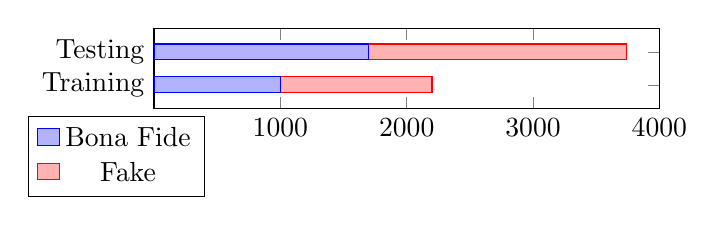
\begin{tikzpicture}
        \begin{axis}[
            xbar stacked, xmin=0, xmax=4000,
            width=8cm,height=2.6cm,
            bar width=2mm,
            xtick={1000,2000,3000,4000},
            xticklabels={1000, 2000, 3000, 4000},
            symbolic y coords={Training,Testing},
            ytick=data,enlarge y limits={abs=3mm},
            legend style={
                at={(-0.25,-0.6)},
                anchor=west,
            }
        ]
            \addplot coordinates { (1000,{Training}) (1700,{Testing})};
            \addplot coordinates { (1200,{Training}) (2040,{Testing})};
            \legend{Bona Fide, Fake}
        \end{axis}
    \end{tikzpicture}

\vspace{-8mm}
\caption{Fingerprint Image Count}
\label{fig:dataset}
\end{wrapfigure}

\noindent
Usually training and validating data are split differently and with relations almost flipped as compared to the dataset provided for LivDet2017 participants.
A train/test split of about 2:1 is often recommended.
Machine learning algorithms get more accurate the more unique data for testing purposes is provided.
Therefore the lack of training data will prove to be an additional challenge.

\begin{wrapfigure}[7]{r}{0.50\textwidth}
    \vspace{-5mm}
    \begin{table}[htb]
    \centering

    \begin{minipage}[r]{0.25\textwidth}
        \centering Training Data (37\%)
        
        \smallskip
        \begin{tabular}{ l r } \hline
            Material    & Share \\ \hline
            Live        & 45\%  \\
            Body Double & 18\%  \\
            Ecoflex     & 18\%  \\
            Wood Glue   & 18\%  \\ \hline
        \end{tabular}
    \end{minipage}
    \hspace{10mm}
    \begin{minipage}[r]{0.25\textwidth}
        \centering Testing Data (63\%)
        
        \smallskip
        \begin{tabular}{ l r } \hline
            Material        & Share \\ \hline
            Live            & 45\%  \\
            Gelatine        & 18\%  \\
            Latex           & 18\%  \\
            Liquid Ecoflex  & 18\%  \\ \hline
        \end{tabular}
    \end{minipage}

    \caption{Material Distribution}
\end{table}

\end{wrapfigure}

\smallskip\noindent
About half (45\%) of both datasets are bona fide fingerprints which leaves the other half comprised of materials emulating human skin.
Different materials were used to train and to validate the neural networks.
Body Double Ecoflex and Wood Glue (each 18\%) were use to train and Gelatine, Latex and Liquid Ecoflex (also each 18\%) are used for validation.
59\% of fingerprint samples are from female subject while 41\% are from males.
Each image was also classified with an age as well.

\begin{wrapfigure}[10]{r}{0.5\textwidth}
    \vspace{-5mm}
    
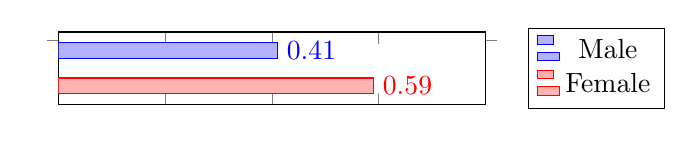
\begin{tikzpicture}
    \begin{axis}[
        xbar, xmin=0, xmax=0.8,
        width=7cm,height=2.5cm,
        bar width=2mm,
        symbolic y coords={F,M},
        ytick=data,enlarge y limits={abs=1mm},
        nodes near coords,
        yticklabels={,},
        xticklabels={,},
        legend style={
            at={(1.1,0.5)},
            anchor=west,
        }
    ]
        \addplot coordinates { (0.41,{M}) };
        \addplot coordinates { (0.59,{F}) };
        \legend{Male, Female}
    \end{axis}
\end{tikzpicture}
\vspace{-5mm}
\caption{Sex Distribution}
    \vspace{2mm}\hrule\vspace{2mm}
    \begin{tikzpicture}
    \begin{axis}[
        height=25mm,
        width=95mm,
        yticklabels={},
        xtick={21, 25, 31.3, 40, 77},
        xticklabels={21, 25, 31.3, 40, 77}]

        \addplot+ [
            boxplot prepared={
                box extend=0.6,
                whisker extend=1,
                lower whisker=19.0, 
                lower quartile=21.0,                
                median=25.0,
                upper quartile=40.0,
                upper whisker=77.0,
                average=31.3
            }
        ] coordinates {};
    \end{axis}
\end{tikzpicture}
\vspace{-2mm}
\caption{Age Distribution}
\label{img:age-dist}

\end{wrapfigure}%

\medskip\noindent
No recognizable variance in prediction accuracy is expected as the diffrence in sex and age do not infer a significant change in fingerprint anatomy or appearance to play a role in this experiment.
With that said, a more mature finger can have noticable damage like scars or common wear from labor and general use.

\begin{wrapfigure}[9]{r}{0.35\textwidth}
    \vspace{-10mm}
    \begin{minipage}[r]{0.15\textwidth}
        \includegraphics[width=\linewidth]{live.bmp}
        \caption{Bona Fide Fingerprint}\label{fig:finger-live}
    \end{minipage}
    \begin{minipage}[r]{0.15\textwidth}
        \includegraphics[trim=32 32 32 32,clip,width=\linewidth]{live.bmp}
        \caption{Sweat Glands}\label{fig:sweat-glands}
    \end{minipage}
\end{wrapfigure}%

\medskip\noindent
All images were captured on a Green Bit DactyScan84C and have a resolution of 500x500 pixel.
The scanner is a standalone high-end device able to capture the fingerprints in high resolution and keeping important details intact.
Bona fide fingerprint images are of such high quality that sweat glands are visible as small white spots on fingerprint ridges in some samples as illustrated in Figure \ref{fig:sweat-glands}.

\medskip\noindent
Training and validation datasets use different materials to fake a fingerprint which adds a level of unpredictablity to the experiment.
Important to note is that none of the used material groups share a distinct property or feature which would make it easier for the trained algorithms to infer the artificiality of unknown materials.

\medskip\noindent
Below is a fingerprint image from each material group.
None of the materials capture sweat glands which my be beneificial to determince whether the presented image is a presentation attack or genuine.

\begin{figure}[!htb]
    \begin{minipage}[r]{0.5\textwidth}
    \begin{minipage}[r]{0.3\textwidth}
        \centering
        \includegraphics[width=\linewidth]{fake-ecoflex.bmp}
        \vspace{-10mm}\caption{Ecoflex}
    \end{minipage}
    \begin{minipage}[r]{0.3\textwidth}
        \centering
        \includegraphics[width=\linewidth]{fake-body-double.bmp}
        \vspace{-10mm}\caption{Body Double}
    \end{minipage}
    \begin{minipage}[r]{0.3\textwidth}
        \centering
        \includegraphics[width=\linewidth]{fake-wood-glue.bmp}
        \vspace{-10mm}\caption{Wood Glue}        
    \end{minipage}
    \caption{Training Dataset}
\end{minipage}
\vrule
\begin{minipage}[r]{0.5\textwidth}
    \begin{minipage}[r]{0.3\textwidth}
        \centering
        \includegraphics[width=\linewidth]{fake-gelatine.bmp}
        \vspace{-10mm}\caption{Gelatine}
    \end{minipage}
    \begin{minipage}[r]{0.3\textwidth}
        \centering
        \includegraphics[width=\linewidth]{fake-latex.bmp}
        \vspace{-10mm}\caption{Latex}
    \end{minipage}
    \begin{minipage}[r]{0.3\textwidth}
        \centering
        \includegraphics[width=\linewidth]{fake-liquid-ecoflex.bmp}
        \vspace{-10mm}\caption{Liquid-Ecoflex}        
    \end{minipage}
    \caption{Validation Dataset}
\end{minipage}
\end{figure}


\newpage


\subsection{Data Acquisition}
\begin{wrapfigure}[13]{r}{10cm}
    \begin{tikzpicture} 
    \begin{umlcomponent}[x=-3,y=0]{Keras} \end{umlcomponent}
    \begin{umlcomponent}[x=3,y=0]{TensorFlow} \end{umlcomponent}

    \umlassemblyconnector[interface=Low Level API]{Keras}{TensorFlow}

    \begin{umlcomponent}[x=2,y=-3]{cnnpad}
        \umlsimpleclass{CnnWrapper}
    \end{umlcomponent}
    
    \umlVHVassemblyconnector[interface=CNN Model Abstractions]{cnnpad}{Keras}


    \umlprovidedinterface[interface=CLI,distance=3cm, with port]{cnnpad}
\end{tikzpicture}
\end{wrapfigure}
Keras is an open-source framework for neural networks and machine learning for the programming language Python.
It offers a simple interface to complex calculations, sophisticated computational resource management and is built on top of TensorFlow (indircite https://keras.io/).

LOOK  HERE Various Python scripts are created for each sequence of the experiment.
Training the networks, saving the trained weights and evaluating the results is done by one pipeline.
Another set of scripts reevaluates best-case trained models and refines the data into human friendly structures.




\subsection{Methodology}
The experiment is split into two parts.
During the first phase the best-case (highest average validation accuracy) for each network needs to be determined.
Due to randomized initial values and subsequent variance in training evolution, the resulting validation accuracy can fluctuate to some degree.
Repetitive training and evaluating will give a set of models for each network which can be serialized and stored.

Models are trained using the provided training dataset over four epochs, which delivered the best balance between validation accuracy and training time.

A total of ten trainings for each network will be used as a pool to pick the best performing model.

\noindent
Trained models are not volatile and can be loaded from disk at any time, so using the best case for each is the fairest approach to make sure every network has the best chances.


\medskip\noindent
Further experiments are conducted in the second phase where the best-case models for each network predicts whether a fingerprint presentation is bona fide or an artificially constructed fingerprint replica.
Unlike neural network training, the predictions of the trained model are static and will not change.
The resulting predictions are used to analyze possible correlations between input data and predicted values.

Just like the original paper about the LiveDet2017 competition, the predictions of each algorithm will be classified by assuming that prediction values of at least 0.50 (cite LiveDet2017) suggest a bona fide fingerprint while all lower values suggest a presentation attack.



\section{Experiment}
\subsection{Phase 1.1 - Frozen Training}

Each network was trained ten times over the course of three hours resulting in a representatively distributed set of trained networks.
Figure \ref{fig:frozen_training_times} visualizes the relations between the average training times.

\begin{tikzpicture}
\begin{axis}[
    ybar,
    width=0.8\linewidth, height=50mm,
    ymax=270,
    ytick=\empty,
    bar width=2mm,
    ymajorgrids,
    ylabel={Average Training Time (s)},
    extra y ticks={30, 60, 90, 120, 180, 240},    
    xtick=data,
    symbolic x coords={EfficientNetB0, InceptionResNetV2, MobileNet, NASNetLarge, ResNet50V2, VGG16, Xception},
    nodes near coords,
    nodes near coords style={/pgf/number format/.cd,precision=0},
    x tick label style={rotate=-45,anchor=west}
    ]
    \addplot table [y={avgtme}]{\frozentrainingtable};
\end{axis}
\end{tikzpicture}

No linear relation between parameter count and training time can be determined.
NasNetLarge takes by far the longest to train with an average of approximately 3.5 minutes. 
MobileNet was the fastest to train with slightly under 30 seconds.


\begin{tikzpicture}
\begin{axis}[
    ymode=log,
    width=0.7\linewidth, height=50mm,
    log basis y=10,
    grid=major,
    boxplot/draw direction=y,
    scale only axis,            
    legend style={
        at={(1.00,0.5)},
        anchor=west},
    ytick=\empty,
    ymax=1,
    ylabel={Validation Accuracy},
    extra y ticks={0.25, 0.5, 0.6, 0.7, 0.8, 0.9},
    extra y tick labels={25\%, 50\%, 60\%, 70\%, 80\%, 90\%},
    xtick=\empty,
    extra x ticks={1, 2, 3, 4, 5, 6, 7, 8, 9, 10, 11},
    extra x tick labels={efficientnet, inceptionresnetv2, mobilenet, mobilenetv2, mobilenetv3, nasnetlarge, nasnetmobile, resnetv2, vgg16, vgg19, xception},
    extra x tick style={
        grid=major,
        tick label style={rotate=-45,anchor=west}}]

        \pgfplotstablegetrowsof{\frozentrainingtable}
        \pgfmathtruncatemacro\TotalRows{\pgfplotsretval-1}
        \pgfplotsinvokeforeach{0,...,\TotalRows}{
            \addplot+[
            boxplot prepared from table={
                table=\frozentrainingtable,
                row=#1,
                lower whisker=min_acc,
                upper whisker=max_acc,
                average=avg_acc
            },
            boxplot prepared,
                % to get a more useful legend
                area legend
            ]
            coordinates {};
        }
\end{axis}
\end{tikzpicture}



Many networks hover around 90\% validation accuracy for their best case.
The earliest insight is that light-weight, small networks are up to par with bigger, much more complex implementations in the context of this experiment.
An additional amount of parameters does not seem to indicate better prediction accuracy for binary classifications.
Even smaller networks can get the same or a better average validation accuracy.

InceptionResnetV2 has a high accuracy fluctuation between training sessions which could not be attributed to any superficial property and the reason behind it is unclear.
On average the aforementioned network performed the worst while being the second largest.

After the training phase, the best-case networks were identified using the average validation accuracy.
The weights for each node are persisted and can be downloaded and applied to reproduce the predictions.
The following analysis will feature these persisted models.


\subsection{Phase 1.2 - Liquid Training}
All networks are trained again with the same configuration, but now all layers are able to adapt their parameters.
Immediately noticeable is the drastic increase in training time for each network.
Another important fact is the increase in resource consumption of unfrozen layers during the training phase.
The workstation was crashing multiple times during training iterations with variations of out-of-memory exceptions.
Figure \ref{fig:liquid_training_times} visualizes the relations between the average training times once again.


\begin{tikzpicture}
\begin{axis}[
    ybar,
    width=0.8\linewidth, height=50mm,
    ymin=0,ymax=2640,
    ytick=\empty,
    bar width=2mm,
    ymajorgrids,
    ylabel={Average Training Time (s)},
    extra y ticks={300, 600, 1200, 1800, 2400},
    extra y tick labels={5min, 10min, 20min, 30min, 40min},
    xtick=data,
    symbolic x coords={efficientnet, inceptionresnetv2, mobilenet, mobilenetv2, mobilenetv3, nasnetlarge, nasnetmobile, resnetv2, vgg16, vgg19, xception},
    nodes near coords,
    nodes near coords style={/pgf/number format/.cd,precision=0},
    x tick label style={rotate=-45,anchor=west}
    ]
    \addplot table [y={avg_tme}]{\liquidtrainingtable};
\end{axis}
\end{tikzpicture}


NasNetLarges training time increased tenfold and it takes almost 40 minutes on average.


\begin{tikzpicture}
\begin{axis}[
    ymode=log,
    width=0.7\linewidth, height=40mm,
    log basis y=10,
    grid=major,
    boxplot/draw direction=y,
    scale only axis,            
    legend style={
        at={(1.00,0.5)},
        anchor=west},
    ytick=\empty,
    ymax=100,
    ylabel={Validation Accuracy},
    extra y ticks={25, 50, 60, 70, 80, 90},
    extra y tick labels={25\%, 50\%, 60\%, 70\%, 80\%, 90\%},
    xtick=\empty,
    extra x ticks={1, 2, 3, 4, 5, 6, 7, 8, 9, 10, 11},
    extra x tick labels={EfficientNetB0, InceptionResNetV2, MobileNet, NASNetLarge, ResNet50V2, VGG16, 
Xception},
    extra x tick style={
        grid=major,
        tick label style={rotate=-45,anchor=west}}]

        \pgfplotstablegetrowsof{\liquidtrainingtable}
        \pgfmathtruncatemacro\TotalRows{\pgfplotsretval-1}
        \pgfplotsinvokeforeach{0,...,\TotalRows}{
            \addplot+[
            boxplot prepared from table={
                table=\liquidtrainingtable,
                row=#1,
                lower whisker=minacc,
                upper whisker=maxacc,
                average=avgacc
            },
            boxplot prepared,
                % to get a more useful legend
                area legend
            ]
            coordinates {};
        }
\end{axis}
\end{tikzpicture}



The increased time spent for a more thorough training phase was worth it as almost all networks now break the 90\% validation accuracy barrier.
InceptionResnetV2 delivers a respectable top accuracy after the disappointing result in the last section.


\begin{table}[htb]
\centering

    \begin{tabular}{ l  r  r  r } \hline
    Network Name       & frozen & delta    & liquid \\ \hline 
    efficientnet       & 90.29  &  +3.0\%  & 93.10 \\
    inceptionresnetv2  & 66.39  & +29.6\%  & 94.33 \\
    mobilenet          & 89.63  &  +2.0\%  & 91.44 \\
    nasnetlarge        & 78.88  & +12.4\%  & 90.05 \\
    resnetv2           & 84.41  &  +7.2\%  & 90.99 \\
    vgg16              & 89.47  &  -2.2\%  & 87.57 \\
    xception           & 78.58  & +17.6\%  & 95.32 \\ \hline 
    \end{tabular}

    \caption{Difference in Top Validation Accuracy}
    \label{tbl:training_diff}
\end{table}


Table \ref{tbl:training_diff} shows the relative gain in validation accuracy of frozen versus freely trained networks.
Many of the smaller networks do not gain much, but on the other hand, InceptionResnetV2 and Xception are now much more competitive.
Xceptions best validation accuracy is comprabale with some of the algorithms handed in during the LivDet2017 competition in regards to the dataset this experiment uses. \cite{LIVDET}

\hfill

\subsection{Phase 2 - Prediction Analysis}
Serialized models are loaded and the testing dataset will be interpreted once again while capturing confidence values for further analysis.
The detection error trade-off curve confirms that none of the networks have a clear advantage compared to each other, but shows that NasNet Large and NasNet Mobile performed the worst with an average difference of TBD \% and TBD \% respectively.



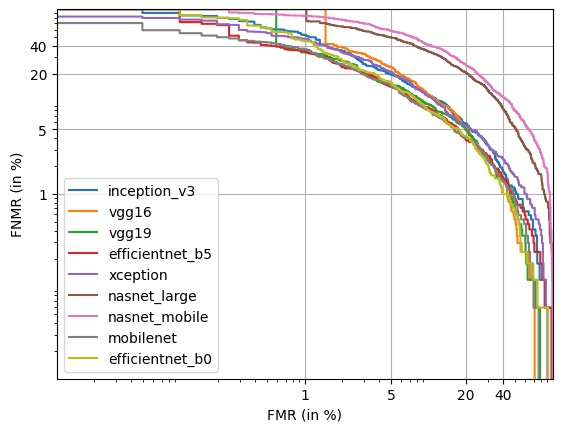
\includegraphics[width=\linewidth]{det-all.jpg}


In the following subsections, each network will be inspected individually by evaluating the performance implicitly assuming a neutral FNMR and FMR rate balancing false positives and false negatives.
This allows the performance to be differentiated in terms of certain materials.


\newpage
\subsubsection{EfficientNet B0}
Even before unfreezing all layers EfficientNetB0 was providing a usable PAD detection accuracy.
Only a small increase in accuracy could be gained by liquid training.
Interestingly the correct non-match rate increased by almost 6\% while the correct match rate sank slightly.

Prediction latencies are consistent, but the few outliers make the average time quite a lot higher than the median latency as seen in Table \ref{tbl:efficientnet_latencies}.

\predictiontables{EfficientNetB0}


\subsubsection{Inception Resnet V2}
A surprising increase in prediction accuracy of almost 30\% was observed for InceptionResnetV2.
The detection scores for all materials benefitted from the liquid training.
Liquid Ecoflex was already reliably detected by the network but is now detected more reliably.
The network gained significant detection capabilities for all other materials.

An average latency of 60ms is slow compared to the other networks.

\predictiontables{InceptionResNetV2}


\subsubsection{MobileNet}
Not a lot improved for MobileNet by unfreezing the layers and in case of Gelatine some accuracy was lost.
Bona fide fingerprints were correctly detected with an accuracy of 91.7\% and 94.4\%, while attack presentations were detected correctly with 87.9 and 89.0\%.

With the relatively inaccurate detection comes the shortest latency with an average of 27ms.
MobileNet was the fastest network in this experiment to deliver a prediction result.

\predictiontables{MobileNet}


\subsubsection{Nasnet Large}
Liquid Ecoflex samples were correctly classified most of the time with a high average rate of 99.7\% after the unfrozen training.
The high attack presentation detection is unfortunately paired with a low correct match rate of only 80\% after unfrozen training, which is the lowest in the entire experiment.

With an average of almost 73ms NasNetLarge has the highest prediction latency.

\predictiontables{NASNetLarge}


\subsubsection{Resnet V2}
Liquid Ecoflex samples were again correctly classified most of the time with a similar rate of 99.1\% after liquid training.
CMR and CNMR are more balanced and result in an overall better accuracy in comparison to NasNetLarge.
The average prediction latency is half of NasNetLarges.

\predictiontables{ResNet50V2}


\subsubsection{VGG16}
The liquid training resulted in a drastic decrease of bona fide fingerpint recognition and compared to that only a minor increase in correct non-match rate was gained.
VGG16 is the only network that lost accuracy after liquid training.

\predictiontables{VGG16}


\subsubsection{Xception}
The best performer in the test has a correct non-match rate of 97.5\% and returns a prediction result in under 36ms, which is quite fast in comparison to the other networks.
Presentation attacks were able to be detected precisely with a max delta of under 1\%.

\predictiontables{Xception}




\endinput





\subsubsection{EfficientNet B0}

The only CMR over 90\% is achieved by EfficientNet B0 which is the second best performer over all.
Bona fide fingerprints were correctly detected with an accuracy of 92.5\%.

\predictiontables{efficientnet}



\medskip
Out of the three tested neural networks MobileNet was performing the best on average thanks to it's high true negative detection rate.
The other two networks however have a better true positive rate.
\bigskip\hrule



\subsection{MobileNet}
Bona fide fingerprints were correctly detected with an accuracy of 89.1\%, while presentation attacks were detected correctly with 93.19\%.
None of the materials show significant variance from each other and are within a range of 92.0\% and 94.7\%.
Liquid Ecoflex shows the worst deception potential.


\predictiontables{mobilenet}




\subsection{Nasnet Mobile}

With a CMR of 81.2\% Nasnet Mobile is the worst performer in the small network group.
The presentation attack detection for the Latex datasets was with only 63\% slightly better than randomly assigned outcomes.
A low precision in regards to the materials provide an interesting difference of over 20\% accuracy between Latex and Liquid Ecoflex.



\medskip
Out of the three tested neural networks MobileNet was performing the best on average thanks to it's high true negative detection rate.
The other two networks however have a better true positive rate.
\bigskip\hrule



\subsection{Xception}
    Presentation attack were able to be detected precicely with a max delta of 2.9\% and all accuracies are over 90\%.
    The overall performance is nothing outstanding and is in line with the median.




\subsection{Inception V3}

    The performance is very similar to the previous network with the accuracies differing by only 0.08\%.
    Inception V3s bona fide detection is a little better, but in turn resentation attacks a bit worse in comparison.




\subsection{EfficientNet B5}

    The highest correct non-match rate in the entire series is held by EfficientNet B5 with 96.03\% which is up to par with specialized solutions (cite livdet2017, p7).
    EfficientNet B5 is the best performer on average in the medium size category but the other two networks are very close in accuracy.

Networks in the midrange size deliver as strong performance and are precise in their accuracies.
EfficientNet B5 has the second best accuracy as well as the best CNMR.

\bigskip\hrule


\subsection{NASNet Large}
\begin{minipage}[c]{0.7\textwidth}
    More than a fifth of all predictions were incorrect which makes NASNet Large not suitable to enhance the quality of fingerprint presentation attack detection mechanisms.
    With almost 18.2\% of difference between Latex and Liquid Ecoflex, the precision is the worst among all tested networks.

    \medskip\centering Match Rates: 
    \begin{tabular}{ r  r  r  r |}
        CMR       & CNMR      & FNMR     & FMR     \\
        80.11\%   & 79.41\%   & 20.59\%  & 19.89\%  \\
    \end{tabular} \hspace{2mm} Accuracy: 79.73\%
\end{minipage}
\hfill
\begin{minipage}[t]{0.3\textwidth}
    \centering
    
\begin{tabular}{ c   r }
    Live               &  80.1\% \\ \hline\hline
    Latex\_02           & 70.6\% \\
    Latex\_01           & 71.2\% \\
    Gelatine\_02        & 77.1\% \\
    Gelatine\_01        & 80.9\% \\
    Liquid\_Ecoflex\_02 & 87.9\% \\
    Liquid\_Ecoflex\_01 & 88.8\%
\end{tabular}
\end{minipage}



\subsection{VGG16}
\begin{minipage}[c]{0.7\textwidth}
    The second largest network in this test did not deliver any outstanding data.
    Accuracy and precision are certainly respectable and in the better half of all tested networks, but unremarkable considering the size and prediction latency.

    \medskip\centering Match Rates: 
    \begin{tabular}{ r  r  r  r |}
        CMR       & CNMR      & FNMR     & FMR     \\
        87.88\%   & 90.29\%   & 9.71\%   & 12.12\%  \\
    \end{tabular} \hspace{2mm} Accuracy: 89.19\%
\end{minipage}
\hfill
\begin{minipage}[c]{0.3\textwidth}
    \centering
    \begin{tabular}{ c   r }
    Live                & 87.9\% \\ \hline\hline
    Latex\_02           & 86.8\% \\    
    Liquid\_Ecoflex\_02 & 88.5\% \\
    Liquid\_Ecoflex\_01 & 89.7\% \\
    Latex\_01           & 91.5\% \\
    Gelatine\_02        & 92.4\% \\
    Gelatine\_01        & 92.9\% \\
\end{tabular}

\end{minipage}



\subsection{VGG19}
\begin{minipage}[c]{0.7\textwidth}
    The largest network provides solid non-match recognition, but cannot provice a good accuracy.
    A CNMR of almost 94\% is the second highest score comparable to algorithms which were handed in for LivDet2017.

    \medskip\centering Match Rates: 
    \begin{tabular}{ r  r  r  r |}
        CMR       & CNMR      & FNMR     & FMR     \\
        86.93\%   & 93.38\%   & 6.62\%   & 13.07\%  \\
    \end{tabular} \hspace{2mm} Accuracy: 90.45\%
\end{minipage}
\hfill
\begin{minipage}[c]{0.3\textwidth}
    \centering
    \begin{tabular}{ c   r }
    Live                & 86.9\% \\ \hline\hline
    Latex\_02           & 90.6\% \\ 
    Liquid\_Ecoflex\_01 & 92.4\% \\
    Liquid\_Ecoflex\_02 & 93.2\% \\
    Latex\_01           & 93.8\% \\
    Gelatine\_02        & 94.7\% \\
    Gelatine\_01        & 95.6\%
\end{tabular}

\end{minipage}


Especially with regards to NASNet Large, the additional size seems to provide no benefit to fingerprint presentation attack-detection mechanisms.
For NASNet Large in particular, the additional size does not provide any benefit to fingerprint presentation attack-detection mechanisms.
VGG16 and VGG18 ware both marginally better than the average network and did not deliver the expected accuracy or precision.

\section{Interpretation}
Larger networks suffer from a complex set of layers and nodes that come with no benefits and even weakens the purpose as the increased calculation time brings inconvenience to the potential user.
Predictions may be disturbed with noise coming from convolutional layers providing data which has little-to-no use for fingerprint presentation attack-detection.

The extreme counterexample is MobileNet in this experiment.
An impressive overall accuracy coming from a high CNMR make this convolutional neural network a prime starting point for a competitive alternative.
With only 16Mb in size on disk it is small enough to fit on embedded devices as well.

\section{Conclusion}
Considering the increase in complexity as well as training and prediction times that deep learning networks with many parameters such as VGG16 bring, the lack in detection accuracy is contrary to expectations.
The original purpose of these networks is to analyze and classify real world objects and animals which bring an acceptable detection rate for fingerprint presentations, but lack the precision and accuracy for real world applications.
Smaller networks in particular represent a good foundation to fine tune and develop a solution which is better fitting for the job.
By concentrating on the key features of the fingerprint, like sweat glands or the smooth curvature of ridge lines of the imprint, a much more accurate system can be built.

Image classification has many facets, but the underlying principles are the same for all applications.
Transfer learning is a powerful paradigm that can lead to surprising results when introducing the pre-trained models to new use cases.
Given the small training dataset, much more accurate predictions are expected when using more extensive reference data to further optimize results.


